\documentclass[a4paper, 12pt]{report}
\usepackage{cmap}
\usepackage{amssymb}
\usepackage{amsmath}
\usepackage{graphicx}
\usepackage{amsthm}
\usepackage{upgreek}
\usepackage{listings}
\usepackage{setspace}
\usepackage[T2A]{fontenc}
\usepackage[utf8]{inputenc}
\usepackage[normalem]{ulem}
\usepackage{mathtext} % русские буквы в формулах
\newenvironment{Proof} % имя окружения
{\par\noindent{\textit{Доказательство.}\\}} % команды для \begin
{\hfill$\scriptstyle\boxtimes$}
\usepackage[left=2cm,right=2cm, top=2cm,bottom=2cm,bindingoffset=0cm]{geometry}
\usepackage[english,russian]{babel}
\usepackage[unicode]{hyperref}
\usepackage{pythonhighlight}
\newcommand\Norm[1]{\left\| #1 \right\|}
\newcommand{\dif}{\mathrm{d}}
\newcommand{\Rm}{\mathbb{R}}
\newcommand{\Cm}{\mathbb{C}}
\newcommand{\Z}{\mathbb{Z}}
\newcommand{\I}{\mathbb{I}}
\newcommand{\N}{\mathbb{N}}
\newcommand{\rank}{\operatorname{rank}}
\newcommand{\Ra}{\Rightarrow}
\newcommand{\ra}{\rightarrow}
\newcommand{\FI}{\Phi}
\newcommand{\Sp}{\text{Sp}}
\renewcommand{\leq}{\leqslant}
\renewcommand{\geq}{\geqslant}
\renewcommand{\alpha}{\upalpha}
\renewcommand{\beta}{\upbeta}
\renewcommand{\gamma}{\upgamma}
\renewcommand{\delta}{\updelta}
\renewcommand{\varphi}{\upvarphi}
\renewcommand{\tau}{\uptau}
\renewcommand{\lambda}{\uplambda}
\renewcommand{\psi}{\uppsi}
\renewcommand{\mu}{\upmu}
\renewcommand{\omega}{\upomega}
\renewcommand{\d}{\partial}
\renewcommand{\xi}{\upxi}
\renewcommand{\epsilon}{\upvarepsilon}
\newtheorem*{theorem}{Теорема}
\newtheorem*{cor}{Следствие}
\newtheorem*{lem}{Лемма}
\begin{document}
\section*{Понятие комплексного числа. Арифметические операции.}
Среди множеств чисел  существует следующая иерархия:
$$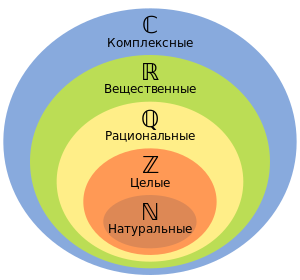
\includegraphics[scale=0.5]{pic1.png}$$
Среди уравнений, которые мы решали на множестве действительных чисел, мы сталкиваемся с уравнением $$x^2 + 1 = 0.$$
Насколько нам известно, на множестве действительных чисел такое уравнение решений не имеет. Однако если всё-таки стоит вопрос о том, чтобы найти какое угодно решение этого уравнения, то как поступить? Было введено обозначение $$i = \sqrt{-1}.$$
$\bullet$ \textit{\textbf{Комплексным числом} называется выражение вида $z = a+bi$, где $a, b \in \mathbb{R}$ (действительные
	числа), а $i$ --- символ, называемый \textbf{мнимой единицей}. При этом число $a$ называется \textbf{действительной частью} $z$ (Обозначение: $a = Re(z)$), а число $b$ --- \textbf{мнимой частью} $z$ (Обозначение: $b = Im(z)$).}\\\\
Множество комплексных чисел обозначается символом $\mathbb{C}$.\\\\
Если $b=0, a\ne 0$, то число $a + 0\cdot i$ считается \textbf{совпадающим с действительными числом} $a$, то есть $a + 0\cdot i = a$.\\\\
Если $b\ne 0, a\ne 0$, то число называется \textbf{мнимым}. Если при $a = 0$, то число $0+bi$ называется \textbf{чисто мнимым} и обозначается через $bi$, то есть ($0+bi = bi$).\\\\
Пусть $z_1 = a_1 + b_1 i$, $z_2 = a_2 + b_2 i$ --- два комплексных числа. Комплексные числа $z_1$ и $z_2$ \textbf{равны}, если равны их действительные и мнимые части, то есть $z_1 = z_2 \Longleftrightarrow a_1 = a_2,\ b_1 = b_2$.\\\\
$\bullet$ \textit{\textbf{Суммой комлексных чисел} $z_1$ и $z_2$ называется число: $$z_1 + z_2 = (a_1 + a_2) + (b_1 + b_2) i.$$}
\textbf{\textit{Свойства сложения комплексных чисел:}}\begin{enumerate}
	\item $z_1 + z_2 = z_2 + z_1$. \begin{Proof}
		$z_1 + z_2 = (a_1 + a_2) + (b_1 + b_2) i = (a_2 + a_1) + (b_2 + b_1) i = z_2 + z_1$.
	\end{Proof}
	\item $(z_1 + z_2) + z_3 = z_1 + (z_2 + z_3)$.
\end{enumerate}
Операция сложения порождает операцию вычитания:\\\\
$\bullet$ \textit{\textbf{Разностью комплексных чисел} $z_1$ и $z_2$ называется число: $$z_1 - z_2 = (a_1 - a_2) + (b_1 - b_2) i.$$ }
$\bullet$ \textit{\textbf{Произведением комплексных чисел} $z_1$ и $z_2$ называется число: $$z_1 \cdot z_2 = (a_1 \cdot a_2 - b_1 \cdot b_2) + (a_1 \cdot b_2 + b_1 \cdot a_2) i.$$ }\\\\
\textbf{\textit{Свойства произведения комплексных чисел:}}\begin{enumerate}
	\item $z_1\cdot z_2 = z_2\cdot z_1$.
	\item $(z_1\cdot z_2)\cdot z_3 = z_1\cdot (z_2\cdot z_3)$.
	\item $(z_1 + z_2)\cdot z_3 = z_1\cdot z_3 + z_2 \cdot z_3$.
\end{enumerate}
Операция умножения комплексных чисел порождает операцию деления:\\\\
$\bullet$ \textit{\textbf{Частным от деления комплексных чисел} $z_1$ и $z_2$ называется число $z_3$ такое, что $z_2 \cdot z_3 = z_1$. }\\\\
Тогда \begin{multline*}
	\dfrac{z_1}{z_2} = \dfrac{a_1 + b_1 i}{a_2 + b_2 i} = \text{[домножим на сопряженное]} = \dfrac{(a_1 + b_1 i)(a_2 - b_2 i)}{(a_2 + b_2 i)(a_2 - b_2 i)}=\\= \dfrac{a_1\cdot a_2 + b_1 \cdot b_2}{a_2^2 + b_2 ^ 2} + \dfrac{b_1 \cdot a_2 - a_1 \cdot b_2}{a_2^2 + b_2^2}i.
\end{multline*}
Иначе говоря, определение комплексных чисел можно сформулировать следующим образом.\\\\
$\bullet$ \textit{Под \textbf{множеством комплесных чисел} $\Cm$ понимают множество упорядоченных пар $(a,b)$ вещественных чисел таких, что на этом множестве введены 3 операции}\begin{enumerate}
	\item $(a_1,b_1) = (a_2,b_2) \Longleftrightarrow a_1 = a_2, b_1 = b_2$;
	\item $(a_1,b_1) + (a_2, b_2) = (a_1+a_2, b_1 + b_2)$;
	\item $(a_1, b_1)\cdot (a_2,b_2) = (a_1a_2 - b_1b_2, a_1b_2 + a_2b_1)$.
\end{enumerate}
Если числа $z_1$ и $z_2$ действительные, то операции сложения и умножения этих чисел совпадают с операциями сложения и умножения действительных чисел.\\\\
Пусть $z = a+ bi$ --- комплексное число.\\\\
$\bullet$ \textit{Комплексное число $\overline{z} = a - bi$ называется \textbf{сопряжённым для комплексного числа $z$}.}\\\\
\textbf{\textit{Свойства сопряжённых комплексных чисел:}}\begin{enumerate}
	\item $z + \overline{z} = 2\cdot a$.\\
	$z - \overline{z} = 2\cdot b\cdot i$.\begin{Proof}
		Если $z = a + bi$, то $z + \overline{z} = (a+bi) + (a-bi) = (a+a) + (b-b)i = 2a$.
	\end{Proof}
	\item $\overline{z_1} + \overline{z_2} = \overline{z_1 + z_2};\ \overline{z_1} - \overline{z_2} = \overline{z_1 - z_2}$.\begin{Proof}
		Пусть $z_1 = (a_1 + b_1i),\ z_2 = a_2 + b_2 i \Rightarrow z_1 + z_2 = (a_1 + a_2) + (b_1 + b_2) i$. Тогда $\overline{z_1} + \overline{z_2} = (a_1 - b_1i) + (a_2 - b_2 i) = (a_1 + a_2) - (b_1 +b_2) i = \overline{z_1 + z_2}$.
	\end{Proof}
	\item $\overline{z_1}\cdot\overline{z_2} = \overline{z_1\cdot z_2}$.\\\\
	$\dfrac{\overline{z_1}}{\overline{z_2}} = \overline{\left(\dfrac{z_1}{z_2}\right)}$.
\end{enumerate}
$\bullet$ \textit{Форма вида $z = a + bi$ называется \textbf{алгебраической формой записи комплексного числа.}}











\section*{Комплексная плоскость. Тригонометрическая и экспоненциальная
	форма записи комплексного числа.}
Пусть на плоскости задана прямоугольная система координат $Oxy$. Каждому комплексному числу вида $z = a + bi$ поставим в соответствие координаты $(a,b)$. С другой стороны, каждой точке с координатами $(a, b)$ мы можем поставить в соответствие комплексное число $z = a + bi$.
$$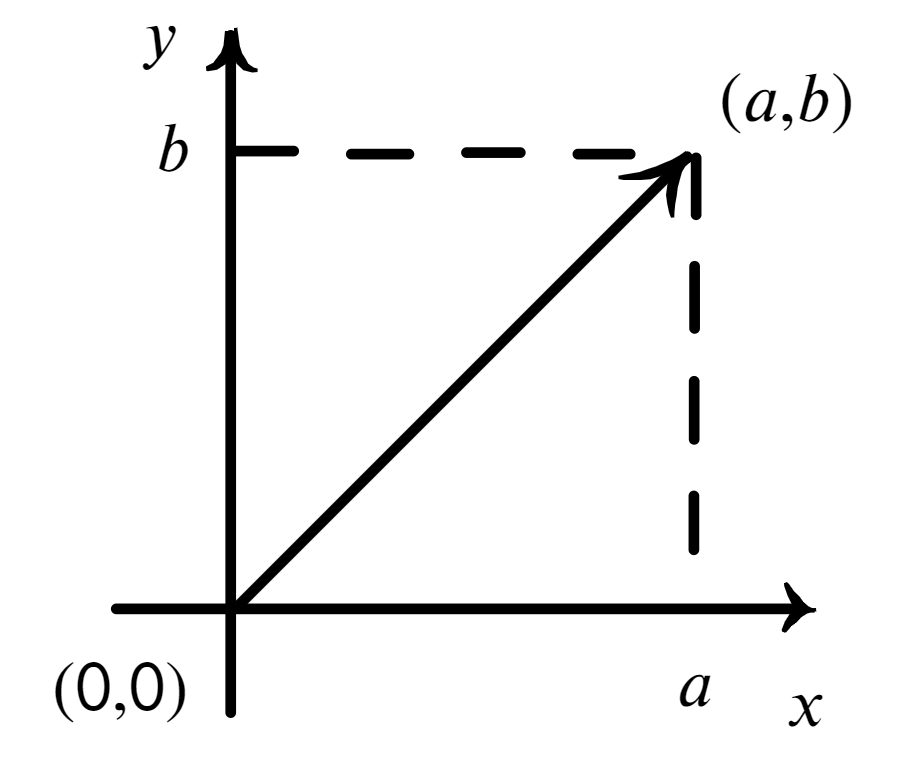
\includegraphics[scale=0.3]{pic2.png}$$
$\bullet$ \textit{Число $\sqrt{a^2 + b^2} = |z|$ называется \textbf{модулем} комплексного числа.}\\\\
Геометрически это расстояние от начала координат до точки, соответствующей комплексному числу.\\
\noindent
\parbox[b][4.5cm][t]{95mm}{
	$\bullet$ \textit{Угол, который образует вектор к числу $z$ с осью $x$ называется \textbf{аргументом} комплексного числа и обозначается $\varphi = \arg (z)$.}\\\\
	Причем, если вращение вектора от оси $x$ против часовой стрелки, то аргумент считаем положительным. Иначе отрицательным.
}
\hfill
\parbox[b][5cm][t]{70mm}{
	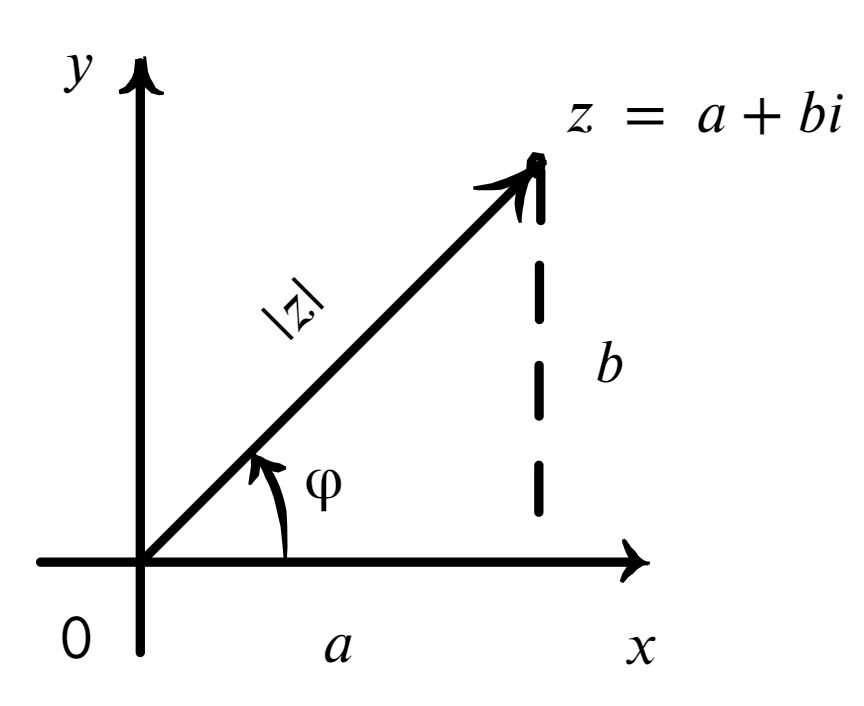
\includegraphics[scale=0.38]{pic3.png}}\\
Значение аргумента можно найти из следующих формул:
$$\cos\varphi = \dfrac{a}{\sqrt{a^2 + b^2}},\quad \sin\varphi = \dfrac{b}{\sqrt{a^2 + b^2}},\quad \tg \varphi = \dfrac{b}{a}.$$
Если $\varphi$ --- аргумент, то чиcла $\varphi + 2\pi k$, $k\in \Z$ также являются аргументами (то есть аргумент определен неоднозначно). Обозначаем \begin{itemize}
	\item $\operatorname{Arg}(z) = \varphi + 2\pi k$ --- все значения аргумента;
	\item $\arg (z) = \varphi$ --- одно значение аргумента.
\end{itemize}
Чаще всего $\varphi \in (-\pi; \pi]$. Но иногда удобно считать, что $\varphi \in [0;2\pi)$.\\\\
$\bullet$ \textit{Это фиксированное значение $\arg (z)$ аргумента  называется \textbf{главным значением аргумента} комплексного числа.}\\\\
Таким образом, $a = |z|\cos \varphi$, $b = |z|\sin\varphi$. Тогда можно записать $$z = a + bi = |z|\cdot (\cos \varphi + i\sin\varphi).$$
$\bullet$ \textit{Такая форма записи комплексного числа называется \textbf{тригонометрической формой записи}}.\\\\
\textbf{\textit{Свойства значения аргумента:}}\begin{enumerate}
	\item $|z| = |\overline{z}|, Arg(z) = -Arg(\overline{z})$.
	\item $|z|^2 = z\cdot\overline{z}$.\begin{Proof}
		Пусть $z = a + bi$, тогда $\overline{z} = a - bi$.\\
		$z\cdot\overline{z} = (a+bi)(a-bi) = a^2 - (bi)^2 = a^2 + b^2 = |z|^2$.
	\end{Proof}
	\item \textit{Модуль разности комплексных чисел равен расстоянию между точками на комплексной плоскости, соответствующих этим числам, то есть $$|z_1 - z_2| = \sqrt{(a_1 - a_2)^2 + (b_1 - b_2)^2}.$$}
	\item $|z_1\cdot z_2| = |z_1|\cdot|z_2|$.\\
	$Arg(z_1\cdot z_2) = Arg(z_1) + Arg(z_2).$
	\item $\left | \dfrac{z_1}{z_2} \right | = \dfrac{|z_1|}{|z_2|}, Arg(\dfrac{z_1}{z_2}) = Arg(z_1) - Arg(z_2)$.
	\item \textbf{Формула Маувра}\\
	\textit{Если $z = |z|(cos\varphi + i\cdot sin\varphi)$, то} $$z^n = |z|^n(cos(n\varphi) + i\cdot sin(n\varphi)).$$
\end{enumerate}
$\bullet$ $e^{i\varphi}=cos\varphi + i\cdot sin\varphi$ --- \textit{\textbf{формула Эйлера}}.\\
$\bullet$ $z = |z| e^{i\varphi}$ ---\textit{ \textbf{экспоненциальная форма записи комплексного числа}}.





\section*{Извлечение корня из комплексного числа.}
Пусть $z$ --- некоторое комплексное число.\\\\
$\bullet$ \textit{\textbf{Корнем n-ой степени из комплексного числа} $z$ называется число $z_0$ такое, что $z_0$ в степени $n$ равно Самому комплексному числу $z$. То есть $z_0^n = z$.}
\newtheorem*{t6_3_1}{Теорема}\begin{t6_3_1} Извлечение корня $n$-ой степени из комплексного числа $z = |z|(cos\varphi + i\cdot sin\varphi)$ всегда возможно и, при $z\ne 0$, даёт
	ровно $n$ различных значений: $$z_k = \sqrt[n]{|z|}\left(cos\left (\dfrac{\varphi + 2\pi k}{n}\right ) + i\cdot sin\left(\dfrac{\varphi + 2\pi k}{n}\right) \right),\ k=0,1,\dots,n-1,$$
	где $\sqrt[n]{|z|}$ --- действительное положительное число, $n$-ая степень которого равна $|z|$.
\end{t6_3_1}
\section*{Разбор задач.}
\begin{center}
	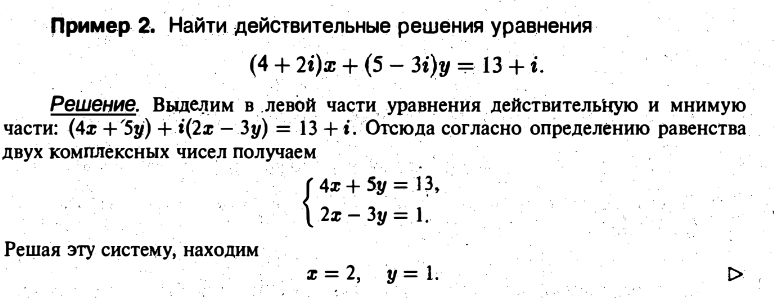
\includegraphics[scale=1.1]{pic5.png}\\
	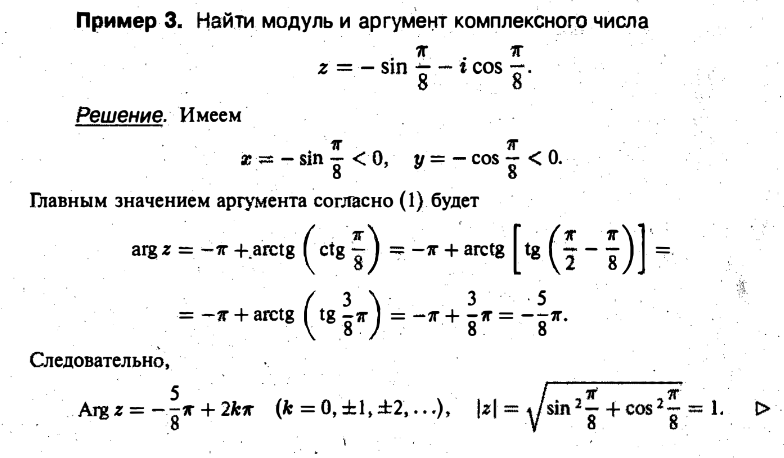
\includegraphics[scale=1.1]{pic6.png}\\
	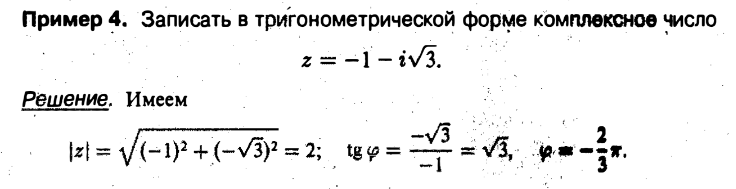
\includegraphics[scale=1.1]{pic7.png}\\
	
\includegraphics[scale=1.1]{pic8.png}\\
	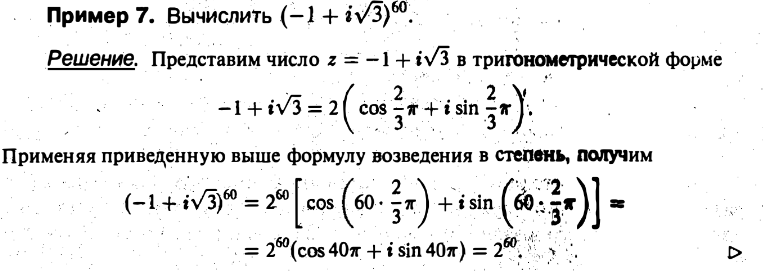
\includegraphics[scale=1.1]{pic9.png}\\
	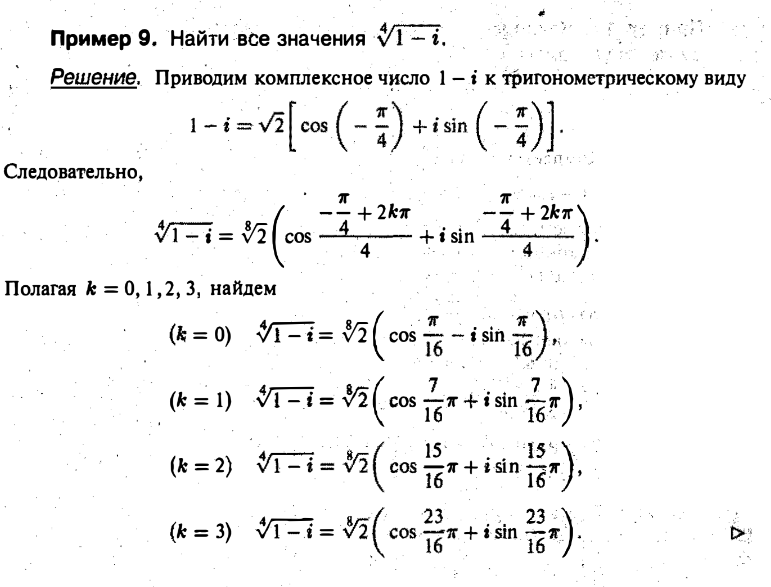
\includegraphics[scale=1.1]{pic10.png}
\end{center}
\end{document}